\documentclass[12pt]{article}

\usepackage[a4paper,margin=2cm]{geometry}

\usepackage{amsmath}
\usepackage{amssymb}
\usepackage{mathtools}

\usepackage{listings}

\usepackage{booktabs} % For tables
\usepackage[table,xcdraw]{xcolor} % For tables

\usepackage{enumerate}
\usepackage{enumitem}

\usepackage{nameref}

\usepackage{xcolor}

\definecolor{codegreen}{rgb}{0,0.6,0}
\definecolor{codegray}{rgb}{0.5,0.5,0.5}
\definecolor{codepurple}{rgb}{0.58,0,0.82}
\definecolor{backcolour}{rgb}{0.95,0.95,0.92}

\lstdefinestyle{mystyle}{
    backgroundcolor=\color{backcolour},
    commentstyle=\color{codegreen},
    keywordstyle=\color{magenta},
    numberstyle=\tiny\color{codegray},
    stringstyle=\color{codepurple},
    basicstyle=\ttfamily\footnotesize,
    breakatwhitespace=false,
    breaklines=true,
    captionpos=b,
    keepspaces=true,
    numbers=left,
    numbersep=5pt,
    showspaces=false,
    showstringspaces=false,
    showtabs=false,
    tabsize=2
}

\lstset{style=mystyle}

\DeclarePairedDelimiter\abs{\lvert}{\rvert}
\DeclarePairedDelimiter\Abs{\lVert}{\rVert}

\usepackage{fancyhdr}

\pagestyle{fancy}
\lhead{\today}
\chead{Exercise 03\\Algorithmic Foundations of Data Science}
\rhead{Fabian Grob\\Simon Michau\\Til Mohr}

\setlength{\headheight}{50pt}

\begin{document}

\section*{Exercise 1}
\begin{enumerate}[label=(\alph*)]
	\item	Using Theorem 3.6:
			\begin{align*}
				\Pr_{T ~ \mathcal{D}^m} &\left( \forall h \in \mathcal{H}: \abs{err_T(h) - err_D(h)} \leq \epsilon \right) > 1 - \delta \\
				\Pr_{T ~ \mathcal{D}^m} &\left( \forall h \in \mathcal{H}: \abs{err_T(h) - err_D(h)} \leq \epsilon \right) > 0.9 \\
				\Rightarrow &\delta = 0.1 \\\\
				m &\geq \frac{1}{2\epsilon^2} \log \left( \frac{2\abs{\mathcal{H}}}{\delta} \right) \\
				143 &\geq \frac{1}{2\epsilon^2} \log \left( \frac{2 \cdot 2^3}{0.1} \right) \\
				143 &\geq \frac{1}{2\epsilon^2} (\log(2^4) - \log(0.1)) \\
				143 &\geq \frac{1}{2\epsilon^2} (4 - \log(0.1)) \\
				\epsilon^2 &\geq \frac{(4 - \log(0.1))}{143 \dot 2} \\
				\abs{\epsilon} &\geq \sqrt{\frac{(4 - \log(0.1))}{286}} \\
				\Rightarrow &\epsilon \geq \sqrt{\frac{(4 - \log(0.1))}{286}} \\
				\epsilon &\geq \sqrt{\frac{(4 - \log(0.1))}{286}} \\\\
				\Pr_{T ~ \mathcal{D}^m} &\left( \forall h \in \mathcal{H}: \abs{err_T(h) - err_D(h)} \leq \epsilon \right) > 0.9 \\
				\Pr_{T ~ \mathcal{D}^m} &\left( \forall h \in \mathcal{H}: \abs{0.03 - err_D(h)} \leq \sqrt{\frac{(4 - \log(0.1))}{286}} \right) > 0.9 \\
				\Rightarrow &err_D(h) \leq 0.03 + \sqrt{\frac{(4 - \log(0.1))}{286}} \simeq 0.05560114718 \simeq 0.06
			\end{align*}
	\item	Using Theorem 3.4:
			\begin{align*}
				\Pr_{T ~ \mathcal{D}^m} &\left( \forall h \in \mathcal{H}: \text{if $h$ is consistent with $T$, then } err_D(h) \leq \epsilon \right) 1 - \delta \\
				\Pr_{T ~ \mathcal{D}^m} &\left( \forall h \in \mathcal{H}: \text{if $h$ is consistent with $T$, then } err_D(h) \leq 0.01 \right) 0.9 \\
				\Rightarrow &\epsilon = 0.01, \delta = 0.1 \\\\
				m &\geq \frac{1}{\epsilon} \ln \left( \frac{\abs{\mathcal{H}}}{\delta} \right) \\
				m &\geq \frac{1}{0.01} \ln \left( \frac{2^3}{0.1} \right) \\
				m &\geq 100 (\ln(3) - \ln(0.1)) \sim 100 \cdot 3.40119738166 = 340.1197 \\
				\Rightarrow &m \geq 341
			\end{align*}
\end{enumerate}

\section*{Exercise 2}
\begin{enumerate}[label=(\alph*)]
	\item
	\item
\end{enumerate}

\section*{Exercise 3}
\begin{enumerate}[label=(\alph*)]
	\item
	\item
\end{enumerate}

\section*{Exercise 4}
\begin{enumerate}[label=(\alph*)]
	\item
	\item
\end{enumerate}

\section*{Exercise 5}
\begin{enumerate}[label=(\alph*)]
	\item	\lstinputlisting{code/exercise_05_output.txt}
	\item	This is due to the fact, that $p_3^{(3)} \neq p_1^{(1)}$.
\end{enumerate}

\section*{Exercise 6}
\begin{enumerate}[label=(\alph*)]
	\item	\begin{enumerate}[label=(\roman*)]
				\item	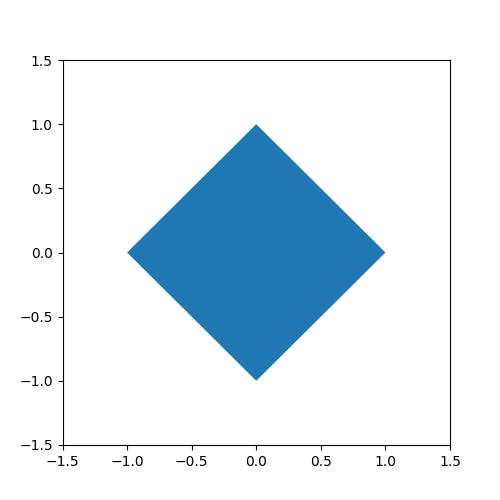
\includegraphics{code/exercise_06_a.png}
				\item	Similarly to how in $l=2$ the ``corners'' of the unit circle are the 2 unit vectors and their negations (so 4 in total), the ``corners'' of the unit circle in $l=3$ are the 3 unit vectors and their negations (so 6 in total). Combined with the edges and facing connecting them they make for a ``diamond'' shape.
			\end{enumerate}
	\item	$vol(B_1^2) = (\sqrt{1^2+1^2})^2 = 2$ and $vol(B_1^3) = 2 \cdot \frac{(\sqrt{1^2+1^2})^2 \cdot 1}{3} = \frac{4}{3}$
	\item	Cover $B_1^l$ by $2k$ cylinders. The thickness of the cylinders is $t \coloneqq \frac{1}{k}$. Thus, the radius of the $i$th cylinder above (or below) is $r_i \coloneqq 1 - (i-1) \cdot t$. Therefore, the volume of the $i$th cylinder is $t \cdot r_i^{l-1} \cdot vol(B_1^{l-1})$. Thus:
			\begin{align*}
				vol(B_1^l) &\leq 2 \sum_{i=1}^k t \cdot r_i^{l-1} \cdot vol(B_1^{l-1}) \\
				&= \left( 2 \sum_{i=1}^k \frac{1}{k} \left( 1 - \frac{i-1}{k} \right) ^ {l-1} \right) \cdot vol(B_1^{l-1}) \\
				&= \left( 2 \sum_{i=0}^{k-1} \frac{1}{k} \left( 1 - \frac{i}{k} \right) ^ {l-1} \right) \cdot vol(B_1^{l-1}) \\
				&= \left( 2 \frac{1}{k} \left( 1^{l-1} + (1 - \frac{1}{k})^{l-1} + \dots + (1 - \frac{k-1}{k})^{l-1} \right) \right) \cdot vol(B_1^{l-1}) \\
				&= \left( 2 \left( \frac{k^{l-1}}{k^l} + (\frac{(k-1)^{l-1}}{k^l}) + \dots + (\frac{1^{l-1}}{k^l}) + (\frac{0^{l-1}}{k^l}) \right) \right) \cdot vol(B_1^{l-1}) \\
				&= \left( 2 \underbrace{\sum_{i=0}^{k} \left( \frac{i^{l-1}}{k^l} \right)}_{\coloneqq S} \right) \cdot vol(B_1^{l-1})
			\end{align*}
			We can use the ratio test on the series $S$:
			\begin{align*}
				\lim_{k \rightarrow \infty} \abs{\frac{\left( \frac{(i + 1)^{l-1}}{k^l} \right)}{\left( \frac{i^{l-1}}{k^l} \right)}} = \abs{\frac{i+1}{i} ^ {l-1}} = \abs{(1 + \frac{1}{i}) ^ {l-1}} > 1
			\end{align*}
			\textbf{Huh? Something is wrong here}
\end{enumerate}

\section*{Appendix}\label{appendix}

\end{document}